\documentclass[sttt,final]{svjour}
% relevant options: draft, referee, final
%
%\usepackage{latexsym}
\usepackage{graphicx}
%\usepackage{amssymb}
%\usepackage{amsfonts,amsmath}
\usepackage{amsbsy}
\usepackage[T1]{fontenc}
\usepackage{url}
\usepackage{xspace}
\usepackage{listings}
\usepackage{xcolor}

\definecolor{darkgrey}{RGB}{64,64,64}
\lstdefinelanguage{SPARK}{
  language = [95]Ada,
  morekeywords = {
    pre,post,assert,
    pragma,
    loop_variant,loop_invariant,contract_cases,
    increases},
  comment=[l][commentstyle]{--\ },
  texcl=true,
  showstringspaces=false
}
\lstdefinestyle{tinystyle}
   {basicstyle=\footnotesize\ttfamily,
    keywordstyle=\scriptsize\color{darkgrey}\pmb,
    commentstyle=\rmfamily\it,
    captionpos=b,
    caption={},label={},
    numbers=none,
    escapeinside={(*}{*)},
    columns=fixed,
    basewidth=0.5em,
  }

\lstset{language=SPARK}
\lstset{style=tinystyle}

%
\newcommand{\DO}{\textsc{do-178}}
\newcommand{\DOB}{\textsc{do-178b}}
\newcommand{\DOC}{\textsc{do-178c}}
\newcommand{\hilite}{Hi-Lite}
\newcommand{\gnatprove}{GNATprove\xspace}
\newcommand{\oldspark}{SPARK~2005\xspace}
\newcommand{\newspark}{SPARK~2014\xspace}
\newcommand{\ada}{Ada\xspace}
\newcommand{\adatwtw}{Ada~2012\xspace}

\newcommand{\etc}{\textit{etc.}\xspace}
\newcommand{\ie}{\textit{i.e.,}\xspace}
\newcommand{\adhoc}{\textit{ad hoc}\xspace}
\newcommand{\Eg}{\textit{E.g.,}\xspace}
\newcommand{\eg}{\textit{e.g.,}\xspace}
\newcommand{\etal}{\textit{et al.}\xspace}
\newcommand{\wrt}{w.r.t.\xspace}
\newcommand{\aka}{a.k.a.\xspace}
\newcommand{\resp}{resp.\xspace}

\begin{document}
%
\title{\newspark\ and \gnatprove}
\subtitle{A Competition Report from Builders of an Industrial-Strength Verifying Compiler}
\author{Duc Hoang\inst{1} \and Yannick Moy\inst{2} \and Angela Wallenburg\inst{3}
}                     % Do not remove
\institute{Ecole Polytechnique F\'ed\'erale de Lausanne, \email{duc.hoang@epfl.ch}
  \and AdaCore, \email{yannick.moy@adacore.com}
  \and Altran~UK, \email{angela.wallenburg@altran.com}}

\date{Received: date / Revised version: date}
% The correct dates will be entered by Springer
%
\maketitle
%
\begin{abstract}
  Extensive and expensive testing is the method most widely used for
  gaining confidence in safety-critical software. With a few
  exceptions, such as SPARK, formal verification is rarely used in
  industry due to its high cost and level of skill required. The grand
  challenge of building a \emph{verifiying compiler} for static formal
  verification of programs aims at bringing formal verification to
  non-expert users of powerful programming languages. This challenge
  has nurtured competition and collaboration among verification tool
  builders; an example is the VerifyThis competition
  \cite{VerifyThis2012}. In this paper we describe our approach to
  popularising formal verification in the design of the
  \newspark\ language and the associated formal verification tool
  \gnatprove. In particular, we present our solution to combining
  tests and proofs, which provides a cost competitive way to develop
  software to standards such as \DO.  At the heart of our technique is
  executable contracts, and the ability to both test and prove
  those. We use running examples from the VerifyThis 2012 competition
  and discuss the results of using our tools on those problems.
\end{abstract}
%
\section{Introduction}
\label{intro}
High quality software, or low defect software, is often costly to
develop. This is a common experience in safety critical systems
development, whether the development is driven by standards such as
\DO, or by any other need to create highly reliable and long-lived
software. Today, extensive and expensive testing is the primary method
used to gain confidence in such software.

The computing research community has been occupied for decades with
the grand challenge of (building) \emph{the verifying compiler}
\cite{Hoare03theverifying}:
%
\begin{quote} A verifying compiler uses mathematical and logical reasoning
  to check the correctness of the programs that it compiles. The
  criterion of correctness is specified by types, assertions, and
  other redundant annotations associated with the code of the
  program. The compiler will work in combination with other program
  development and testing tools, to achieve any desired degree of
  confidence in the structural soundness of the system and the total
  correctness of its more critical components.
\end{quote}

As predicted in \cite{Hoare03theverifying}, this grand challenge has
called for co-operation among research teams and it has encouraged
and benefited from competition. An example of such beneficial
competition is the VerifyThis competition, which is the context of
this report.

Great strides have been made in proof automation. At present,
so-called ``push-button'' static program verification is achievable for some
substantial classes of industrial programs. New programming language
features for program verification have been explored and theoretical
models of complex existing language features have been devised to
increase the reasoning capabilities for mainstream programming
languages. See \cite{HatcliffLLMP12} for many insights in the
programming language approach to program verification. However, there
are still many remaining challenges before we can expect verifying
compilers to be as widely used as testing.

Formal software verification has been successfully used and scaled to
large industrial projects \cite{Woodcock2009,vcc2009}. While many case
studies have been successful, few formal methods have reached the
take-up and maturity level where industrial non-experts continue to
use the method for project after project, and where this formal
method is a permanent part of the business of industrial software
development. There are some notable exceptions: for example, the SPARK
language and toolset for static verification has been applied for many
years in on-board aircraft systems, control systems, cryptographic
systems, and rail systems \cite{sparkbook2012,oneill2012}.

We identify two main hurdles that currently hinder the
take-up of verifying compiler technology:
%
\begin{enumerate}
\item difficulty in reaching non-expert users, and
\item lack of convincing cost-benefit argument.
\end{enumerate}
%
In this paper we will describe our approach to solving these two
problems in the design of the \newspark\ language and the associated
formal verification tool \gnatprove. We will use running examples from
the VerifyThis 2012 competition and discuss the results of using our
tools on those problems.

This paper is organised as follows: first we describe the key language
features of \newspark, which is a complete update of the \oldspark\
language and tools. \newspark has been designed with many lessons
learned from the programming language and verification community, and
naturally from experiences in industrial use of \oldspark. Then in
section \ref{hilite} we describe our unique integration of testing and
proving, which was developed in the collaborative research project
\hilite\ \cite{hiliteERTS2012} between Altran (formerly Praxis),
AdaCore, and Inria. In the resulting new tool architecture the
compiler and the verifier are based on the same front-end
\cite{ksd2012}. In section \ref{overflowsemantics} we describe
specific language features which enables specifications to be written
more naturally. In section \ref{automation}, we present GNATprove, our
formal verification tool, and in
section \ref{verifythis} its results in the VerifyThis 2012
competition. We conclude with future work.

\section{Key Language Features for Verification}
\label{langfeatures}

All the functional specification features in \newspark are executable. This
means that their verification can be performed either dynamically, by running
the program, or statically with a dedicated formal verification tool.

\subsection{Ada 2012}

Ada 2012 introduced new language features for facilitating the
specification of programs~\cite{ada2012rationale}, many of which were
inspired from the corresponding features in \oldspark. In the following,
we describe some of these which we used in the solutions for the
VerifyThis 2012 competition challenges.

The most useful of these new features is without doubt the
preconditions and postconditions popularised by the Design-by-Contract
approach~\cite{meyer:1988:OSC}. In challenge~1 (the longest common
prefix problem) we can for example specify that function \verb|LCP|
expects arguments within bounds, and that it returns a bounded
result. Note the use of the new \textit{aspect} syntax in Ada 2012, in
which the declaration of \verb|LCP| is followed by keyword \verb|with|
and a list of aspects.

\begin{lstlisting}
function LCP (A : Text; X, Y : Integer) return Natural with
  Pre  => X in A'Range and then Y in A'Range,
  Post => LCP'Result in 0 .. Index'Last;
\end{lstlisting}

In the postcondition of a function, the new attribute \verb|Result| is
used to refer to the result of the function. The attribute \verb|Last|
represents the last value (upper bound) in the range of type
\verb|Index|. Another new attribute \verb|Old| is used to refer to the
value of some variables on entry to a subprogram. These were used
in solving challenge 2 (the binary tree sum) of the VerifyThis
competition. Note that we use the short-circuit Boolean operator
\verb|and then| for which the second argument is only executed or
evaluated if the first argument is not enough to determine the value
of the expression. This is helpful for example in producing valid
specifications involving partial functions, like
\verb|Y /= 0 and then X / Y|.

The expression of specifications is made easier by new expression
forms in Ada 2012. If-expressions and case-expressions are the
expression forms which correspond to the usual if-statements and
case-statements. Note that an if-expression without else-part
\verb|(if A then B)| expresses a logical implication of \verb|B| by
\verb|A|. Quantified expressions \verb|(for all X in A)| and
\verb|(for some X in A)| correspond to the mathematical universal and
existential quantifications (see Section \ref{overflowsemantics} for
more information about the domain of bound variables). Expression
functions define a function with a single expression, like in
functional programming languages. As expression functions can be part
of the specification of programs (contrary to regular function
bodies), they provide a powerful way to abstract complex parts of
specifications.

\subsection{SPARK 2014}

The new version of SPARK is based on the features of Ada 2012. There
are also new features added, some of which are inspired from
\oldspark. An example is the loop invariant.

Like preconditions and postconditions are essential new features of
Ada 2012 for specification, the loop invariant pragma is essential in
\newspark. A loop invariant can be inserted anywhere in the main list
of statements in a loop, and it expresses the cumulated effect of the
loop up to that point. For example, here is the loop invariant used in
challenge~1:

\begin{lstlisting}
pragma Loop_Invariant
  (for all K in 0 .. L - 1 => A (X + K) = A (Y + K));
\end{lstlisting}

Note that a loop invariant in SPARK has a slightly different semantics
to the classic loop invariant introduced by Hoare
\cite{hoare69cacm}. A classic loop invariant has to hold when reaching
the loop, at the start of each iteration of the loop, and when exiting
the loop. A SPARK loop invariant only has to hold when execution
reaches the corresponding program point. Essentially the loop
invariant is like an assert except it also acts as a cut point in
formal verification. A cut point means that the prover is free to
forget all information about modified variables that has been
established within the loop. Only the given Boolean expression is
carried forward. For formal verification in SPARK, checks are
generated for initialisation and preservation of the loop invariant,
similarly to the classic approach. The SPARK semantics are easier to
work with for programmers.

In formal verification, it is very common that loop invariants compare
the value of a variable at loop entry and at the n$^{th}$ iteration of
the loop. To enable such specifications, SPARK 2014 introduces the
\verb|Loop_Entry| attribute, which can be applied to such a
variable. We have used that feature in our solution to the binary tree sum
challenge, see Section \ref{verifythis}.

A loop variant pragma has also been defined in SPARK 2014, to express
a quantity varying monotonically at each iteration of the loop. As
loop invariants, a loop variant can appear anywhere in the main list
of statements in a loop. For example, here is the loop variant used in
the longest commmon prefix challenge:

\begin{lstlisting}
pragma Loop_Variant (Increases => L);
\end{lstlisting}

Note that this variant does not take the usual non-negative decreasing
argument. Instead, it takes a list of increasing or decreasing integer
values, bounded by their type in Ada, and the overall order over this
list is the lexicographic order combined with individual
directions. In the example above, there is only one element in the
list, so it should increase at each run through the loop. Like for
loop invariants, the point where this increase matters is the program
point where the loop variant appears in the code. As in the classic
case, the value of the variant is compared against the value at the
corresponding program point in the previous iteration of the loop.

Subprogram contracts can become quite large, even with the use of (expression)
functions to abstract common parts of contracts. Therefore, SPARK 2014 allows
the definition of contracts by cases, similar to behaviours in
JML \cite{JML}. For example, the contract of \verb|LCP| can state separately
sub-contracts for the cases where the elements at \verb|X| and \verb|Y| are
different, or \verb|X| and \verb|Y| are equal. This contract may be used
instead of or in addition to a precondition and a postcondition.

\begin{lstlisting}
function LCP (A : Text; X, Y : Integer) return Natural with
  Contract_Cases =>
    (A (X) /= A (Y) => LCP'Result = 0,
     X = Y          => LCP'Result = A'Last - X + 1,
     others         => LCP'Result > 0);
\end{lstlisting}

Note that the cases above are disjoint and complete, as expected given
the SPARK design goals: one and only one case should be applicable at
every call. The presence of the \verb|others| case ensures the
completeness here.

\section{Integrated Testing and Proving}
\label{hilite}
As we have mentioned, in the development of the new generation
language and toolset \newspark, we have a particular focus on
providing a good cost-benefit argument and on reaching non-expert
users.

We will describe a few observations of what drives the current
practices in the industry, in order to help us with the cost-benefit
argument. We will also see how progress in the research of behavioural
interface specification languages \cite{HatcliffLLMP12} enables an
approach where test and proof can be elegantly integrated.

\subsection{Motivation: Industry Safety Standards and Testing}
Industry standards and certification documents highly influence the
state-of-the-practice safety-critical software development. \DOB\
\cite{do178b} is a document that is used as a basis for certification
of airborne software by institutions such as Federal Aviation
Administration (FAA) and European Aviation Safety Agency
(EASA). Though \DOB\ is for avionics, it is often used in other
safety-critical sectors as well. It is regarded as very successful
within the avionics industry itself; since its introduction in 1992 no
commercial aircraft fatality has been attributed to \DOB-certified
software. The majority of objectives in \DOB\ consider
verification. \DOB\ is non-prescriptive with regards to programming
languages, software tools, particular development processes etc. The
development of requirements-based tests is mandatory, including normal
range tests cases and robustness (abnormal range) test cases. The
standard requires verification of both high-level requirements and
low-level requirements. Three levels of testing are defined in \DOB:
hardware/software integration testing, software integration testing,
and low-level testing - all based on requirements. The test cases must
fully cover the code and all exercised code should be traceable to
requirements. This requires coverage analysis such as MC/DC. Such
structural low-level testing, together with robustness testing is
expensive. For example, a large cost is associated just for collecting
and verifying output of these tests. Our goal is to reduce this cost,
while still meeting the objectives prescribed by the standard.

Formal methods can help to verify that no anomalous behaviour will
occur, for example it can be used to prove the absence of run-time
errors. Formal methods can also be used to show compliance between a
program's actual and intended behaviour. Furthermore, a proof of
program correctness is comparable to exhaustive analysis achieving
100\% coverage. Though formal methods and other kinds of verification
are recognised as beneficial, they do not contribute to \DOB\
certification credit, and their use has had to be justified by other
means. However, \DOC\ \cite{do178c}, the recently released successor and
replacement of \DOB, allows some of the prescribed testing
activities to be replaced by formal methods. From RTCA \cite{do178c}:
%
\begin{quote}
  The use of formal methods is motivated by the expectation that, as
  in other engineering disciplines, performing appropriate
  mathematical analyses can contribute to establishing the correctness
  and robustness of a design.
\end{quote}
%
Formal methods are complementary to testing, and may find faults that
are not detected by testing, but they cannot establish verification
evidence for the target hardware. Therefore testing on the target is
still required. However, formal analysis of source code can be used to
show compliance with the low-level requirements. \DOC\ requires an
argument for property preservation between the source code and the
object code for those properties that have been verified formally at
the source level. Since formal program verification and testing are
complementary, we would like to use each method where it is most
efficient. For this we need to make sure that the combination is at
least as strong as testing alone.

\subsection{Executable Contracts}
Programming using contracts is a way to organise your code. By stating
a precondition and a postcondition of a subprogram as for example in
section \ref{langfeatures}, we assign responsibilities. The subprogram
is responsible for the postcondition to be met, as long as it is
called under the assumptions of its precondition, which it relies
upon. Similarly, a caller of this subprogram is responsible for ensuring that
the precondition of the subprogram holds, before calling it. It can
then rely on the postcondition of the called program upon return. This
programming discipline encourages a modular design of the
software. Furthermore when verification is concerned, this can be done
in a modular fashion as well. Modularity gives the flexibility to
perform verification during development, rather than waiting until
after integration.

In addition to user-defined contracts we also have implicit contracts
given for example by a strong type system such as Ada's and the
signatures of subprograms. For example there is an implicit
precondition that subprogram parameters have values within their types
and likewise an implicit postcondition that guarantees that output
parameters and function results have values allowed by their type. As
an example, consider what difference it makes to the user-supplied
contract, if you would use the type \verb|Natural| instead of
\verb|Integer| for the \verb|Input| parameter of procedure \verb|Sqrt|:

\begin{lstlisting}
procedure Sqrt (Input : Integer; Res: out Natural) with
  Pre  => Input >= 0,
  Post => (Res * Res) <= Input and then
          (Res + 1) * (Res + 1) > Input;
\end{lstlisting}

In this case the implicit precondition would be sufficient and a
user-supplied precondition would not be necessary. Since there is a
cost associated with users writing contracts, there is a benefit in
designing the language so that the basic language features already
provide a rich default contract.

The notion of preconditions and postconditions was first introduced by Hoare
\cite{hoare69cacm}, and later reinvented as Design-by-Contract by Meyer
\cite{meyer:1988:OSC}. Traditionally, contracts have been interpreted quite
differently depending on whether used for formal program verification or for
run-time assertion checking. For formal program verification, assertions have
typically been interpreted as formulae in classical first-order logic. This is
not consistent with the run-time assertion checking semantics.

Much effort has been spent the last decades to popularise formal
program verification. \cite{tseChalin10} did something as unusual as
surveying practitioners, to find that they prefer run-time assertion
checking semantics. Furthermore he developed a semantics to allow
formal executable contracts, i.e. compatible with run-time assertion
checking, in the hope that those users who are already annotating
their code with assert statements, could more easily be convinced to
start writing contracts. Ada 2012 and thus \newspark have such
semantics.

As users can execute contracts, they can also debug them like code, and test
them when formal verification is too difficult to achieve.
Furthermore, there is an advantage in keeping the annotation language
the same, or almost the same, as the programming language: users
don't have to learn one more language. If the contract is also formal,
the entry barrier to formal program verification can be lowered by
making it available to those who would write executable contracts.

\subsection{Mixing Test and Proof}

Low-level requirements, in \DO\ terms, are typically expressed in
natural language at subprogram or unit level. Formal executable
contracts can be used to express those requirements at the
subprogram level. Thanks to the same semantics for test and proof as
we have just discussed, we can use either (or both) of test and proof
to verify a subprogram. Thanks to modular verification, it is then
possible to mix test and proof to use the verification method that is
most cost effective for each module. If the chosen method is testing
the benefits of formal executable contracts are:
%
\begin{itemize}
\item Low-level requirements expressed as contracts
\item Successful execution of postcondition $\rightarrow$ test successful
\item No need to collect and verify output
\item More run-time checks gives better robustness testing
\end{itemize}
If the chosen verification method for a subprogram is proof, the
benefits of formal executable contracts are:
\begin{itemize}
\item Low-level requirements expressed as contracts
\item Successful proof of postcondition $\rightarrow$ low-level
  requirement verified for all input
\item Approach allowed by \DOC\ formal methods supplement
\item Proof of absence of some run-time exceptions provides for some
  robustness testing
\item Proving process faster when annotations can be executed (debugging failed proof attempts is very time-consuming)
\end{itemize}
%
But what about soundness of the mixed approach? When some low-level
requirements are tested and some are proved, remember in
\DOC-terms the combination needs to be as good as if all low-level
requirements were tested.

Central to modular verification is the statement of assumptions and
guarantees. For global correctness, \emph{all} subprograms must
establish their postconditions (under the assumption of their
preconditions), and for \emph{all} calls to a subprogram, its
precondition must be verified by the caller before the call.

In our mixed approach of test and proof, we have these same global
correctness requirements as usual for modular verification. The
difference is that some subprograms may be tested and some be proved,
and we must still make sure that all assumptions are verified. Let us
consider the two cases: 1) a tested subprogram \verb|T| calls a proved
subprogram \verb|P|, and 2) a proved subprogram \verb|P| calls a
tested subprogram \verb|T|. In the first case, when verifying \verb|T|
we must make sure that the precondition of \verb|P| is
established. When testing \verb|T|, this can be done by executing the
precondition of \verb|P|. In the second case, the correctness of
\verb|P| relies on that after having verified the precondition of and
then called \verb|T|, then \verb|T| should return in a state where the
postcondition holds. This assumption on \verb|T| should be verified
when testing \verb|T| by executing the assertion that its postcondition
holds. Both of these verification cases are only possible because we
have executable contracts.

Although we don't describe it here, the same verification by testing of
assumptions made during formal verification needs to be done for implicit
contracts, related to initialization of in-type values and non-aliasing. We
have implemented these additional verifications in the GNAT compiler through
dedicated switches that the user can set~\cite{hiliteERTS2012}.

\subsection{Compiler Implementation}
For \newspark\ we are building the verification tools using the GNAT compiler,
see \cite{ksd2012} for a description and discussion of this architecture. One
advantage here is that the compiler inserts these additional checks needed to
verify at run time assumptions made during proof. Another advantage is that
formal verification has access to the precise configuration of the target
platform used for compilation (size of integers, endianness, \etc), which
facilitates performing proofs that depend on the target.

\section{Choosing the Right Semantics for Integers}
\label{overflowsemantics}
As already mentioned, there has traditionally been a difference in
interpretation of contracts depending on whether used for formal
verification, or for run-time assertion checking. One area where this
difference is of practical significance is in the semantics for
integers. An effect of having the same semantics in assertions as in
the program code, is that run-time exceptions must be considered, and
avoided, in the assertions as well as in the program. As an example,
consider a programmer who wants to state a pre-condition that the
addition of two number fits in a desired integer type:

\begin{lstlisting}
  Pre => X + Y in Some_Integer_Type
\end{lstlisting}

\noindent
The problem is that
\verb|X + Y| itself can cause an arithmetic overflow, and worse this
is not relevant to the correctness of either the program or the
specification. When executable semantics are used for integer
operations in assertions, there will therefore in practical formal
verification tools be a large number of extra proof obligations that do not
point to real issues either in the program code or the assertions. In
traditional assertion languages aimed for formal verification,
mathematical universal integers are used for such operations and proof
can safely proceed without involving the user. Furthermore, user
studies \cite{jotChalin04} show that users who are otherwise happy
with run-time assertion checking semantics, still prefer mathematical
semantics for intermediate integer operations in assertions.

From a user perspective, mathematical semantics for integer operations in
assertions is a good solution. However, for our hybrid verification argument
described in the previous section to work, it is mandatory to have the same
semantics for test and proof. Fortunately, we have the option to implement
a solution for this in the compiler GNAT, which we are building our
verification tools on. Also, the Ada standard supports this approach by not
requiring that the program issues an overflow error when an intermediate value
does not fit into the base type, providing the correct result is computed.

Existing users of \oldspark\ and potential new users of \newspark\
together cover a wide spectrum of strong preferences regarding this
issue. Existing users of \oldspark\ who perform formal verification of
absence of run-time errors for their programs want the traditional
mathematical integers in assertions and executable semantics for the
program. Another user wants the same executable semantics in
assertions and program code, and wants to leave the assertions in the
shipped code. Many users could not have executed code that uses a
library for unbounded integers because of certification and
performance reasons, \etc Because of these strong needs, we provide
three alternative overflow checking modes in GNAT and \gnatprove:
\begin{enumerate}
\item Strict mode: normal overflow checks
\item Minimized mode: larger base type (64bits) used when needed
\item Eliminated mode: use bignum library in the remaining cases
\end{enumerate}
In the second and third cases the compiler performs a simple static
analysis and decides if a larger machine integer, or even an unbounded
one, is needed. This gives a flexible solution, where the user chooses
between 3 modes. The choice is independent for assertions and
code. However, the same choice for execution and formal verification
is required for our hybrid verification with test and proof to be
sound.

There is a potential source of confusion in providing several overflow
checking modes but this is managed with SPARK language profiles. SPARK
users can chose pre-defined profiles and customise their own profile
to prohibit particular language features, and enforce tool settings
such as overflow semantics, according to project-specific constraints
and regulations.

\section{Making Automatic Verification Work}
\label{automation}

As \gnatprove uses the Why3 platform~\cite{why3} to generate VCs and
call provers, it can target as many output formats and automatic or
manual provers as the Why3 platform allows (many!), but we focus on
the automatic proof of VCs through the use of the SMT prover
Alt-Ergo~\cite{altergo} which is distributed with \gnatprove. There
are two steps to make automatic verification work: first make it
possible, then make it efficient.

The choice of source programming language is essential to make
automatic verification possible. On the one hand, it should proscribe
those features which render automatic verification impossible or very
hard, and on the other hand, it should contain enough features which
facilitate the expression of specifications. The former is obtained by
restricting \newspark to a subset of \adatwtw without pointers,
exceptions, aliasing, and effects in expressions. The latter is
obtained by the features introduced in \adatwtw and
\newspark. \adatwtw was specifically designed to include
preconditions, postconditions, type invariants, \etc so that users can
specify arbitrarily complex invariant properties on the data and
control of their programs, and test these properties at run time. As
mentioned, \newspark further adds loop invariants, loop variants, \etc
so that a user can formally prove these properties.

Efficient formal verification relies on a subtle coordination between
the VC generator and the prover, so that the VCs produced can be
efficiently proved. \gnatprove relies heavily on the features of the
Why3 language~\cite{guitton2011boogie} to produce provable VCs. For
example, the VCs are kept small by translating the semantic
dependencies between entities at the Ada source code level into
syntactic inclusions between modules at the Why3 intermediate code
level, and by using the abstraction feature in Why3 for the
intermediate code that checks for absence of run-time errors. This
ensures that the generated VCs only contain relevant definitions and
axioms. As another example, one can choose to produce fewer but more
complex VCs: the default in \gnatprove is that a VC accounts for all
paths leading to an assertion, using an efficient
computation~\cite{leino2005ipl}, instead of generating one VC for each
path leading to an assertion (also available in \gnatprove as an
option). The choice of axiomatisation of Ada data types (integer
types, enumeration types, record types, array types, \etc) in Why3
also has a significant effect on the provability of VCs. We have tuned
these axiomatisations to better suit the mechanisms inside SMT provers
like Alt-Ergo. Similarly, we have tailored the axiomatisation for a
generic library of containers~\cite{dross:2011:tap} to SMT provers.

Finally, modular verification based on pre- and postconditions can
very easily exploit multi-core architectures, as the generation of VCs
for different units, or the proof of different VCs, can both be run in
parallel. Typically, projects contain hundreds of units, and lead to
the generation of thousands of VCs, which can be run by \gnatprove on
as many cores as are available. Note also that \gnatprove uses file
timestamps to avoid re-generating VCs for units which have not been
updated, and file hashes to avoid re-proving VCs that have already
been proved. This is crucial when developing either the code or the
associated annotations, to avoid unnecessary rework.

\section{VerifyThis Competition}
\label{verifythis}
In this section, we will describe our solutions to two of the
challenges from the 2012 VerifyThis competition. The first challenge
is the longest common prefix problem, \verb|LCP|. The second challenge
is a tree sum, \verb|PrefixSum|, which is a binary tree summation
algorithm implemented in-place on an array. For the latter we have one
complete fixed-size solution suitable for automatic verification using
the current prototype version of \newspark\ and
\gnatprove. Furthermore, we have specified a general version of the
\verb|Upsweep| procedure of the second challenge initially using
\oldspark\ as a reference, then translated into \newspark,
experiencing the benefits of executable annotations.
\subsection{Solution to Challenge 1: Longest Common Prefix}

The longest common prefix solution can be readily coded in \newspark
as follows:

\begin{lstlisting}
subtype Index is Positive range 1 .. 1_000_000;
type Text is array (Index range <>) of Integer;

function LCP (A : Text; X, Y : Integer) return Natural with
  Pre  => X in A'Range and then Y in A'Range,
  Post =>
    (for all K in 0 .. LCP'Result - 1 =>
      A (X + K) = A (Y + K))
      and then
    (X + LCP'Result = A'Last + 1
      or else Y + LCP'Result = A'Last + 1
      or else A (X + LCP'Result) /= A (Y + LCP'Result));

function LCP (A : Text; X, Y : Integer) return Natural is
   L : Natural;
begin
   L := 0;
   while X + L <= A'Last
     and then Y + L <= A'Last
     and then A (X + L) = A (Y + L)
   loop
      pragma Loop_Invariant
        (for all K in 0 .. L - 1 =>
          A (X + K) = A (Y + K));
      pragma Loop_Variant (Increases => L);
      L := L + 1;
   end loop;
   return L;
end LCP;
\end{lstlisting}

The type \verb|Text| is an array of integers with unknown bounds. The input
specification that parameters \verb|X| and \verb|Y| are indices in the array
parameter \verb|A| can be expressed as a precondition involving the Ada
attribute \verb|'Range|, and membership tests \verb|X in ...| The output
specification that the result is the length of the longest common prefix
starting at \verb|X| and \verb|Y| can be expressed as a postcondition in two
parts, using the \adatwtw attribute \verb|'Result| to express the function
result:
\begin{itemize}
\item A quantification stating that the subarrays of \verb|A| of length
  \verb|LCP'Result| starting at \verb|X| and \verb|Y| are equal.
\item A disjunction of cases stating that either one of the two
  subarrays reaches the end of array \verb|A|, or the elements
  following the two subarrays in \verb|A| are different. Note here
  that the use of the lazy Boolean connective \verb|or else| is
  compulsory to make sure that \verb|X + LCP'Result| and
  \verb|Y + LCP'Result| are within the bounds of \verb|A| when
  accessing \verb|A| in the last line of the postcondition.
\end{itemize}

Running \gnatprove on this code without loop invariant or loop variant results
in the generation of 13 VCs: 1 VC for the postcondition, and 12 VCs for all
run-time checks (6 array index checks, 5 numeric overflow checks, 1 subtype
range check). All VCs related to run-time checks are proved. These VCs
represent both checks in the code and checks in assertions for the array
accesses in the postcondition. The VC for the postcondition is not proved, due
to the presence of a loop in the body of \verb|LCP|.

Proving the postcondition requires the insertion of a loop invariant in the
body of \verb|LCP|, which expresses that the subarrays of \verb|A| of length
\verb|L| starting at \verb|X| and \verb|Y| are equal. Since \verb|L| is the
value returned by \verb|LCP|, this loop invariant matches the first part of the
postcondition when the loop terminates. As expected, the postcondition is
proved with this additional loop invariant. \gnatprove generates 4 additional
VCs to prove that the loop invariant initially holds at the first iteration
through the loop, that it is maintained by subsequent iterations, and that the
two array accesses in the loop invariant expression are within bounds. All 4
additional VCs are also proved.

Finally, proving termination of \verb|LCP| requires the insertion of a loop
variant in the body of \verb|LCP|, which expresses that the value of \verb|L|
always increases between two consecutive iterations through the loop. Since
\verb|L| is of a bounded type (the scalar type \verb|Natural| of natural
numbers), it cannot be infinitely incremented without failing a run-time
check. Since we have already proved that no run-time check fails in \verb|LCP|,
proving the variant proves the termination of \verb|LCP|. The corresponding VC
is proved by \gnatprove.

The final version of \verb|LCP| is proved in 6s on a laptop with 4G
RAM and a 3GHz processor.

\subsection{Solution to Challenge 2: Tree Sum}

We have chosen to implement an iterative version of prefix sum
instead of a recursive one, which better matches the constraints
commonly found in critical embedded software where recursion is
usually not allowed. In order to make automatic proof possible, we fix
the length of the array to 8. The complete solution is quite long (186
lines of code, not counting empty lines), so we only show here
selected parts. The initial solution without annotations is
straightforward, and only 50 lines long. As an example, here is the
implementation of procedure \verb|Upsweep|:

\begin{lstlisting}
procedure Upsweep (A : in out Input;
                   Output_Space : out Positive) is
   Space : Positive := 1;
   Left  : Natural;
   Right : Natural;
begin
   while Space < A'Length loop
      Left := Space - 1;
      while Left < A'Length loop
         Right     := Left + Space;
         A (Right) := A (Left) + A (Right);
         Left      := Left + Space * 2;
      end loop;
      Space := Space * 2;
   end loop;
   Output_Space := Space;
end Upsweep;
\end{lstlisting}

The postcondition of procedure \verb|Upsweep| states that the array
parameter \verb|A| is put in an intermediate form \wrt its initial
value (denoted \verb|A'Old|). The contract of procedure
\verb|Downsweep| states that it takes as input an array parameter
\verb|A| in an intermediate form \wrt a \verb|Ghost| array parameter,
and that it outputs via the same parameter \verb|A| the desired prefix
sums of array \verb|Ghost|. By calling in sequence \verb|Upsweep| and
\verb|Downsweep| on an array \verb|A|, with the initial value of
\verb|A| passed as \verb|Ghost| parameter, a caller performs the
desired in-place modification of \verb|A|. Although \newspark does not
yet support ghost parameters, which are only used for proofs, this is
the role of parameter \verb|Ghost| here, hence its name.

\begin{lstlisting}
procedure Upsweep (A : in out Input;
                   Output_Space : out Positive) with
  Pre  => All_Elements_In (A, Maximum),
  Post => All_Elements_In (A, 8 * Maximum)
    and then Output_Space = 8
    and then Intermediate_Form (A, A'Old);

procedure Downsweep
  (Ghost : Input; A : in out Input;
   Input_Space : in Positive)
with
  Pre => All_Elements_In (Ghost, Maximum)
    and then All_Elements_In (A, 8 * Maximum)
    and then Input_Space = 8
    and then Intermediate_Form (A, Ghost),
  Post =>
    A (0) = 0
      and then
    A (1) = Ghost (0)
      and then
    A (2) = Ghost (0) + Ghost (1)
      and then
    A (3) = Ghost (0) + Ghost (1) + Ghost (2)
      and then
    A (4) = Ghost (0) + Ghost (1) + Ghost (2) + Ghost (3)
      and then
    A (5) = Ghost (0) + Ghost (1) + Ghost (2) + Ghost (3)
          + Ghost (4)
      and then
    A (6) = Ghost (0) + Ghost (1) + Ghost (2) + Ghost (3)
          + Ghost (4) + Ghost (5)
      and then
    A (7) = Ghost (0) + Ghost (1) + Ghost (2) + Ghost (3)
          + Ghost (4) + Ghost (5) + Ghost (6);
\end{lstlisting}

The function \verb|Intermediate_Form| gives the exact relationship between the
initial value of the array (parameter \verb|B| below) and its intermediate
value between the calls to \verb|Upsweep| and \verb|Downsweep| (parameter
\verb|A| below). We define it as an expression function in \adatwtw, which has
the benefit that \gnatprove automatically generates a postcondition for
\verb|Intermediate_Form| equivalent to its body. We also give a precondition to
\verb|Intermediate_Form| to prove that its evaluation cannot fail run-time
checks (overflow checks and index checks here).

\begin{lstlisting}
function Intermediate_Form (A, B : Input) return Boolean with
  Pre => All_Elements_In (A, Maximum * 8)
    and then All_Elements_In (B, Maximum);

function Intermediate_Form (A, B : Input) return Boolean is
  (for all K in A'Range =>
     (if (K + 1) mod 8 = 0 then
        A (K) = B (0) + B (1) + B (2) + B (3) +
                B (4) + B (5) + B (6) + B (7)
     elsif (K + 1) mod 4 = 0 then
        A (K) = B (K) + B (K-1) + B (K-2) + B (K-3)
     elsif (K + 1) mod 2 = 0 then
        A (K) = B (K) + B (K-1)
     else
        A (K) = B (K)));
\end{lstlisting}

Note that the contracts of all previous procedures and functions contain calls
to function \verb|All_Elements_In|, which returns \verb|True| if all elements
of an array are bounded in absolute value, which we also define as an
expression function:

\begin{lstlisting}
function All_Elements_In (A : Input; Max : Positive)
return Boolean is
   (for all K in A'Range => A (K) in -Max .. Max);
\end{lstlisting}

These specifications add 62 lines to the initial 50 lines for the solution. To
prove them with \gnatprove, we add 84 more lines for loop invariants and loop
variants. As an example, here are the loop invariant and loop variant for the
inner loop of procedure \verb|Upsweep|. Inside the loop invariant,
\verb|A'Loop_Entry| denotes the value of \verb|A| on entry to the loop.

\begin{lstlisting}
pragma Loop_Invariant (
  (Left + 1) mod Space = 0
    and then
  All_Left_Elements_In (A, Left, Space * 2 * Maximum)
    and then
  All_Right_Elements_In (A, Left - 1, Space * Maximum)
    and then
  (Left + 1) mod (Space * 2) = Space
    and then
  (if Left >= A'Length then Left = 8 or Left = 9)
    and then
  (for all K in A'Range =>
    (if K in A'First .. Left - Space
       and then (K + 1) mod (2 * Space) = 0
     then
        A (K) = A'Loop_Entry (K) + A'Loop_Entry (K - Space)
     else
        A (K) = A'Loop_Entry (K))));
pragma Loop_Variant (Increases => Left);
\end{lstlisting}

The final version of prefix sum is partially proved (78 VCs proved, 8 VCs
%
% Florian says this description is not consistent
% unproved) in 138s on a laptop with 24G RAM and 24 processors at 2.4GHz (to
%
unproved) in 138s on a multi-core laptop with 24G RAM at 2.4GHz (to
be able to prove VCs in parallel).  These 8 unproved VCs are either loop
invariants or postconditions, which are not proved automatically due to the use
of the \verb|mod| operator, currently not well handled in the underlying
automatic prover. We have checked all of them manually, and written an expanded
version of loop invariants and intermediate function where all occurrences of
the \verb|mod| operator are replaced by an explicit enumeration of the possible
cases for all indexes, which \gnatprove is able to fully prove automatically.

\subsection{General  Tree Sum}
As mentioned, we chose to implement an iterative version of
\verb|PrefixSum| as a better fit for critical embedded software.
Though the presented complete solution makes automatic
proof possible with the prototype version of our tools,
the specification could be improved. Here we present
a general specification for the simple property of the \verb|Upsweep|
procedure. This solution avoids explicit listing of intermediate state in the
contract, because it is too detailed and hard to judge whether it is
correct, and it would be impossible to use that specification scheme
for a larger array.

The \verb|Upsweep| precondition consists of two parts: 1) the starting
values in the array are within a certain \verb|Maximum|, which is
specified here to be as large as it can be without causing overflows,
and 2) the length of the array is a power of two. The postcondition
state two observations about the algorithm: 1) the even positions are
left unchanged during the upsweep, and 2) upon completion of
\verb|Upsweep|, the last element holds the sum of all the elements in
the array.

We have added a constant \verb|Tree_Depth| for the size of the tree
that fits in the input array. This is to be able to neatly specify an
important precondition on \verb|Upsweep| that the size of the array is
a power of 2. Otherwise the binary tree algorithm is not guaranteed to
work, so we want to be explicit about this precondition. By adding
this constant and precondition we ask the user to effectively fix the
size, but it is done in a general fashion. It is worth noting that
this precondition could have been stated without asking the user to fix
the size, and perhaps more naturally as $\exists n: \mathit{Integer}.~ A'\mathit{Length} = 2^n$, but it is our experience that existential quantification is
difficult for the automatic provers that we have available.

We have added a couple of functions to make the specification
intuitive: \verb|Is_Even|, and more importantly \verb|Summation|, the
mathematical operation for adding a sequence of numbers.

\begin{lstlisting}
Tree_Depth : constant := 3;
Maximum    : constant := Integer'Last / (Index'Last + 1);

function Is_Even (K : Integer) return Boolean is
  (K mod 2 = 0);

function Summation (A : Input; Start_Pos, End_Pos : Index)
return Integer with
  Pre => Start_Pos <= End_Pos;

function Summation (A : Input; Start_Pos, End_Pos : Index)
return Integer is
  (if Start_Pos = End_Pos then
     A (Start_Pos)
   else
     A (End_Pos) + Summation (A, Start_Pos, End_Pos - 1));

procedure Upsweep (A : in out Input;
                   Output_Space : out Positive) with
  Pre  =>
   (for all K in A'Range => A (K) in -Maximum .. Maximum)
      and then
   A'Length = 2 ** Tree_Depth,
  Post =>
   (for all K in A'Range =>
     (if Is_Even (K) then A (K) = A'Old (K)))
    and then
   A (A'Last) = Summation (A'Old, 0, A'Last);
\end{lstlisting}

The downside is that this improved specification does not yet verify
with the current version of \gnatprove. This general specification was
initially developed using \oldspark\ and the existing verification
tools, as a reference example in our development of \newspark\ and
\gnatprove. Using the \oldspark\ verification tools, we could add the
necessary axiom on the summation proof function that the summation of
two adjacent intervals of the array is equal to the summation of the
combined interval. Ideally we would add support for the summation
operation including axioms to \gnatprove\ in the future.

%% Even though we could not currently prove this using \gnatprove, we had
%% a very rewarding experience in moving the example from \oldspark\ to
%% \newspark. Consider the following lengthy two loop invariants. They
%% are longer than they need to be in \newspark\ (due to legacy reasons
%% the loop invariant need to repeat some of the loop conditions).
%% %
%% \begin{lstlisting}
%% package body PrefixSum_General is

%%    procedure Upsweep (A : in out Input; Output_Space : out Positive) is
%%       Space : Positive := 1;
%%       Left  : Natural;
%%       Right : Natural;
%%       A_Old : constant Input := A;
%%    begin
%%       while Space < A'Length loop
%%          Left := Space - 1;

%%          pragma Loop_Invariant
%%            (A'Length mod Space = 0
%%               and then
%%             2 * Space <= A'Length
%%               and then
%%             not Is_Even (Left + Space)
%%               and then
%%             Left < Space
%%               and then
%%             (Left + 1) mod Space = 0
%%               and then
%%             (for all K in A'Range =>
%%               A (K) in -Maximum * Space .. Maximum * Space)
%%               and then
%%             (for all K in A'Range =>
%%               (if Is_Even (K) then A (K) = A'Loop_Entry (K)))
%%               and then
%%             (for all K in A'Range =>
%%               (if (K + 1) mod Space = 0 then
%%                 A (K) = Summation (A'Loop_Entry, K + 1 - Space, K))));
%%          pragma Loop_Variant (Increases => Space);

%%          while Left + Space < A'Length loop
%%             pragma Loop_Invariant
%%               (Left + Space < A'Length
%%                  and then
%%                A'Length mod Space = 0
%%                  and then
%%                2 * Space <= A'Length
%%                  and then
%%                not Is_Even (Left + Space)
%%                  and then
%%                (Left + 1) mod Space = 0
%%                  and then
%%                (for all K in A'Range =>
%%                  (if K < Left then
%%                    A (K) in -Maximum * Space * 2 .. Maximum * Space * 2
%%                   else
%%                    A (K) in -Maximum * Space .. Maximum * Space))
%%                  and then
%%                (for all K in A'Range =>
%%                  (if Is_Even (K) then A (K) = A'Loop_Entry (K)))
%%                  and then
%%                (for all K in A'Range =>
%%                  (if K < Left and (K + 1) mod (Space * 2) = 0 then
%%                    A (K) = Summation (A_Old, K + 1 - Space * 2, K)
%%                  elsif Left <= K and (K + 1) mod Space = 0 then
%%                    A (K) = Summation (A_Old, K + 1 - Space, K)))
%%                  and then
%%                A (Left) = Summation (A_Old, Left + 1 - Space, Left)
%%                  and then
%%                A (Left + Space) = Summation (A_Old, Left + 1, Left + Space));
%%             pragma Loop_Variant (Increases => Left);

%%             Right     := Left + Space;
%%             A (Right) := A (Left) + A (Right);
%%             Left      := Left + Space * 2;
%%          end loop;
%%          Space := Space * 2;
%%       end loop;
%%       Output_Space := Space;
%%    end Upsweep;

%% end PrefixSum_General;
%% \end{lstlisting}
%% %
%% After adding the necessary summation axiom, there would still be two
%% verification conditions remaining unproved. At that point it was very
%% helpful that the loop assertions are also executable. This meant that
%% after running some tests with run-time checking turned on, we could
%% get some confidence in the correctness of the long and complicated
%% loop invariant. This is very valuable since it decreases the time
%% spent on debugging failed proof attempts while finding the correct
%% loop invariant and then to write user rules (axioms) to cover for the
%% incompleteness of the prover.

\subsection{Useful Tool Features}

The format of the competition exercised useful features of \gnatprove,
which helped to find errors early in the code and in the
annotations. The most useful of these features is certainly the
ability to execute annotations, which allows annotations to be tested
and debugged as if they were code. It was used during the competition
to quickly locate the reason for an unprovable VC on challenge 1: the
loop test was using a strict comparison operator instead of the
correct non-strict one. To locate the problem, the participating
author simply wrote a test exercising \verb|LCP| on an input, compiled
it with run-time checks, and executed it. The run-time error raised
precisely located the failing loop invariant. Although this example
was simple enough to immediately understand the underlying problem, it
would have been possible to use the debugger to further investigate
the issue, which can be extremely useful on real industrial code. The
ability to execute annotations was also useful for challenge 2, which
requires the development of complex loop invariants, to quickly
correct erroneous ones. This feature won the prize of user-assistance
tool feature awarded by the jury of the VerifyThis competition.

Another very useful feature for these challenges was the ability to eliminate
completely all possibilities of numeric overflow in annotations, as described
in section~\ref{overflowsemantics}. While using this feature results in only 10
more overflow VCs in challenge 1, which are all proved with the current
annotations, it adds 60 overflow VCs in challenge 2, most of which require
modifications of annotations, or addition of new annotations, to be
proved. Note that this feature is compatible with the execution of annotations,
as compilation also takes into account the overflow mode when compiling
arithmetic expressions.

Various features of \gnatprove make it very convenient to use inside
an Integrated Development Environment (currently GPS, the GNAT
Programming Studio, see Fig.~\ref{fig:snapshot}). The user can choose
to call \gnatprove on a selected file, an individual subprogram, or
even a single line of code. This was key to speeding up the
modify/verify loop during the competition. When a VC is not proved,
the IDE can also display the corresponding statements in the code, to
help figure out why some assertions do not hold on some paths.

More generally, these challenges already make use of numerous
language features in \adatwtw and \newspark that facilitate the
expression of specifications: preconditions and postconditions, loop
invariants and loop variants, special attributes \verb|'Result|,
\verb|'Old| and \verb|'Loop_Entry|, expression functions, quantified
expressions and if expressions.

\begin{figure*}
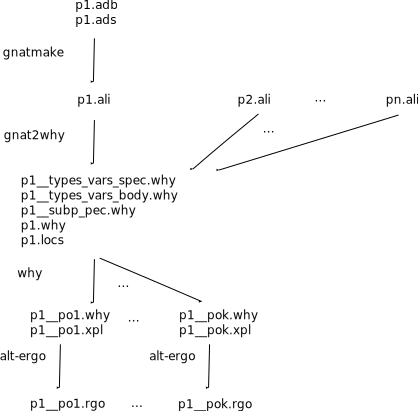
\includegraphics[width=\linewidth]{gnatprove.png}
\caption{Snapshot of GNATprove results on challenge 1 inside GPS}
\label{fig:snapshot}
\end{figure*}

%% \caption Snapshot of GNATprove results on challenge 1 in GPS

\section{Ongoing Work}
\label{ongoing}

\gnatprove is the result of a complete redesign of the SPARK language and
associated tools, which started in 2010 with project \hilite\ \cite{Hi-Lite}.
Altran and AdaCore are collaborating to complete this new version of SPARK by
the start of 2014. On the tool side, current work focuses on flow analysis,
support for investigating unproved VCs, and improvements of the SMT prover.

Flow analysis is the verification of the data dependences of
subprograms. This analysis which has always been a component of SPARK
verification is being redeveloped for \newspark, based on
program dependence graphs~\cite{horwitz:1988:pldi}. An important
novelty is that, while \oldspark requires that the user annotates
programs with data dependence contracts, they are optional in
\newspark, and \gnatprove generates them when not present. A minimal
flow analysis is always required for the soundness of proofs, while a
more complete flow analysis is optional. The minimal flow analysis
ensures that all variables are initialized prior to being read.

Good support in the investigation of unproved VCs is key to making
formal program verification cost-effective in industry. \gnatprove
currently provides various solutions to that problem: the ability to
execute annotations to detect errors in code and/or annotations; the
display of program paths to detect errors or locate missing
annotations; the possibility to call alternate provers to identify
prover shortcomings. In the future, we would like to add the display
of counter-examples generated by the prover, as already provided by
some SMT provers~\cite{CVC3,Z3model}, and in Riposte
\cite{riposteICLP}, a counter-example finder for \oldspark.

We have been exploring two promising ways to improve the results of the
Alt-Ergo SMT prover on the VCs generated in \gnatprove: handling selected
axiomatisations as decision procedures~\cite{dross:2012:smt}, and incrementally
selecting axioms~\cite{cgs09:ipo,kuhlwein:2012:ijcar}. More work is needed to
make these modes the default inside \gnatprove.

\section{Conclusions}
\label{conclusions}
In this paper we have described the key elements of the design of
\newspark and \gnatprove. This design is based on experience over many
years working with both expert and non-expert \oldspark developers in
industry. The design focuses particularly on improving the usability for
non-expert users and providing a convincing cost-benefit argument for
using formal verification in regulated industries. \newspark and
\gnatprove are still being implemented, and it is early days for
\DOC, but early evaluations are very encouraging, and some are
documented in the case study developed by Astrium Space Transportation
\cite{dasia2013}.
%
\bibliographystyle{alpha}
\bibliography{sttt_2013}

\end{document}
